% This text is proprietary.
% It's a part of presentation made by myself.
% It may not used commercial.
% The noncommercial use such as private and study is free
% Sep. 2005 
% Author: Sascha Frank 
% University Freiburg 
% www.informatik.uni-freiburg.de/~frank/
%
% additional usepackage{beamerthemeshadow} is used
%  
%  \beamersetuncovermixins{\opaqueness<1>{25}}{\opaqueness<2->{15}}
%  with this the elements which were coming soon were only hinted
%\documentclass[8pt]{beamer}
\documentclass[10pt]{beamer}
\usepackage{etex}
\newenvironment<>{varblock}[2][\textwidth]{%
  \setlength{\textwidth}{#1}
  \begin{actionenv}#3%
    \def\insertblocktitle{#2}%
    \par%
    \usebeamertemplate{block begin}}
  {\par%
    \usebeamertemplate{block end}%
  \end{actionenv}}
%\usepackage{hyperref}
%\usepackage{natbib}
%\usepackage{beamerthemeshadow}
\usepackage{beamerinnerthemecircles, beamerouterthemeshadow}

\usepackage{amsmath,amssymb,amsfonts}
\usepackage[pdf]{pstricks}
%\usepackage{bbm}
%\usepackage{booktabs}
\usepackage{amsthm}
\usepackage{booktabs}
\usepackage{graphicx}
\usepackage{epsfig}
%\usepackage{graphics}

% MQ: This is to be able to compile on the Riksbank computer. Uncomment with my laptop. Ugly solution but will have to do for now.
%\usepackage{epstopdf}
%\epstopdfsetup{outdir=./}

\usepackage{rotating}

\usepackage{url}
%\usepackage{breqn}
%\usepackage{hyperref}
\usepackage[authoryear]{natbib}
\usepackage{setspace}
\usepackage{multirow}
%\usepackage{harvard}
\usepackage{xcolor}
%\usepackage{multicolumn}
\usepackage{algpseudocode}
\usepackage{sidecap}
\usepackage{bbm} 
\usepackage{courier}
\usepackage{tikz}
\usetikzlibrary{arrows,shapes,snakes,automata,backgrounds,petri}

\tikzset{
  treenode/.style = {align=center, inner sep=0pt, text centered,
    font=\sffamily},
  arn_n/.style = {treenode, circle, white, font=\sffamily\bfseries, draw=black,
    fill=black, text width=1.5em},% arbre rouge noir, noeud noir
  arn_r/.style = {treenode, circle, red, draw=red, 
    text width=1.5em, very thick},% arbre rouge noir, noeud rouge
  arn_x/.style = {treenode, rectangle, draw=black,
    minimum width=0.5em, minimum height=0.5em}% arbre rouge noir, nil
}
\beamertemplatenavigationsymbolsempty

\newenvironment{myenumerate}{\begin{enumerate}[(1)]}{\end{enumerate}} 
\sidecaptionvpos{figure}{c}
% FOR COLORING PARTS  OF TABLE
%\usepackage[beamer,customcolors]{hf-tikz}

%\tikzset{hl/.style={
%    set fill color=red!80!black!40,
%    set border color=red!80!black,
%  },
%}

\mode<presentation> {
    \usetheme{Madrid} %Frankfurt} %Bergen, Berkely, Berlin, Boadilla, CambridgeUS, Darmstadt,
                          %Frankfurt, Goettingen, Singapore, Warsaw
    \usecolortheme{beaver} %seahorse} %default} %beetle, seahorse, wolverine, dolphin, beaver
    %\useoutertheme[subsection=true]{smoothbars} 
    \usefonttheme{default}
    %\usecolortheme{red}
    

	\setbeamercolor{block title}{use=unstructure, fg=white, bg=purple!75!black} %{use=structure,fg=white,bg=purple!75!black}
	%\setbeamercolor{block body}{use=structure,fg=black,bg=white!20!white}    
    %\setbeamercolor{block body}{bg=white}
    \setbeamertemplate{enumerate items}[default]
    \setbeamercolor{enumerate item}{fg=purple!75!black} 
    \setbeamercolor{enumerate subitem}{fg=purple!75!black} 	 
	\setbeamercolor{itemize item}{fg=purple!75!black}  
	\setbeamertemplate{itemize item}[triangle]  
	\setbeamercolor{itemize subitem}{fg=purple!75!black}
	\setbeamertemplate{itemize subitem}[triangle]
	\setbeamertemplate{blocks}[framed]


}



%\usepackage{colortbl}
%\definecolor{yellow}{cmyk}{0,0.18,0.90,0.00}

%\usepackage{xcolor}

%\usepackage[authoryear]{natbib}
\begin{document}
\title[Lecture 3]{Bayesian Learning 732A46: Lecture 3}  
\author[Matias Quiroz]{Matias Quiroz\inst{1}$^{,}$\inst{2}}
\setbeamerfont{institute}{size=\fontsize{7pt}{8pt}}
\institute[LiU and Riksbank]{
  \inst{1}%
   Division of Statistics and Machine Learning, Link\"{o}ping University\\~\\
  \inst{2}%
   Research Division, Sveriges Riksbank\\
     
}

%\institute[Riksbank and LiU]{Sveriges Riksbank and Division of Statistics and Machine Learning, Link\"{o}ping University}

\date[]{April 2016} %\today 

%\usebackgroundtemplate{%
%  \vbox to \paperheight{\vfil\hbox to \paperwidth{\hfil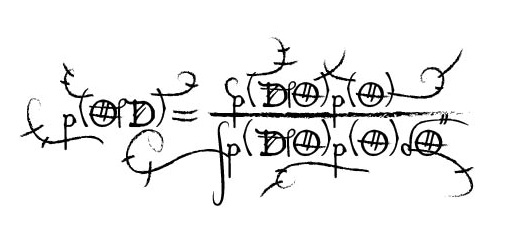
\includegraphics[width=1.5in]{Bayes.jpg}\hfil}\vfil}
%}

{
%\usebackgroundtemplate{\begin{center}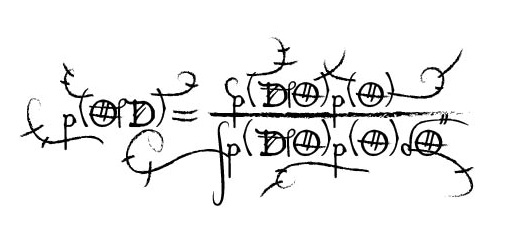
\includegraphics[width=0.4\paperwidth]{Bayes.jpg}\end{center}}
\usebackgroundtemplate{%
  \vbox to \paperheight{\hbox to \paperwidth{\hfil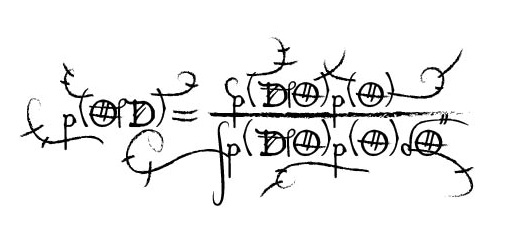
\includegraphics[width=2in]{Bayes.jpg}\hfil}}
}
\begin{frame}
\titlepage
\end{frame}
}
%\frame{\titlepage} 

%\frame{\frametitle{Overview of the talk}\tableofcontents}





\begin{frame}{Lecture overview}

\begin{itemize}
\item Multiparameter models - direct simulation and marginalization. \medskip{}
\item Normal model with unknown variance \medskip{}
\item Multinomial model \medskip{}
\item Multivariate normal with known covariance matrix

%\item Villanis Points:
%\item Multiparameter models
%\item Marginalization
%\item Normal model with unknown variance
%\item Bayesian analysis of multinomial data
%\item Bayesian analysis of multivariate normal data
\end{itemize}
\end{frame}

\begin{frame}{Direct simulation}

\begin{itemize}
\item Once $p(\theta|y)$ is derived we use it for \textbf{posterior analysis}.\medskip{}

\item \textbf{\color{blue}Direct}: \emph{known distribution} - \textbf{Example}: Normal, Beta, Gamma. \medskip{}
\item {\color{blue}Examples} [$\theta \sim p(\theta|y)$ continuous. Replace $\int$ by $\sum$ for discrete $\theta$]
\vspace{1mm}
\begin{itemize}
\item[] {\color{blue}Expectation}: $E(\theta)=\int\theta p(\theta|y)d\theta$
\vspace{1mm}
\item[] {\color{blue}Variance}: $V(\theta)=\int\left(\theta-E(\theta)\right)^2 p(\theta|y)d\theta$
%\item[] {\color{blue}Prediction} : $p(\tilde{y}|y)=\int p(\tilde{y}|\theta) \pi(\theta)d\theta$
\vspace{1mm}
\item[] {\color{blue}Probabilities}: $\Pr(\theta \in A)=\int_A p(\theta|y)d\theta$. \\ E.g. if $A=\{\theta;\theta \in [0,\infty)\}$ then $\Pr(\theta\leq 2)=\int_0^{2}p(\theta|y)d\theta$.
\end{itemize}
\medskip{}
\item {\color{red}Note}: the function of interest is \textbf{{\color{blue}averaged over the posterior uncertainty}} of the parameters. 



\end{itemize}
\end{frame}


\begin{frame}

\frametitle{Direct simulation, cont.}

\begin{itemize}
\item Nothing but expectations of a function $h(\theta)$, i.e. $$E[h(\theta)]=\int h(\theta)p(\theta|y)d\theta.$$
\item {\color{blue}Expectation}: $E(\theta)=\int\theta p(\theta|y)d\theta$. {\color{red} $h(\theta)=\theta$}.
\vspace{1mm}
\item[] {\color{blue}Variance} : $V(\theta)=\int \left(\theta-E(\theta)\right)^2 p(\theta|y)d\theta$. {\color{red} $h(\theta)=\left(\theta-E(\theta)\right)^2$}.
\vspace{1mm}
\item[] {\color{blue}Probabilities}: $\Pr(\theta \in A)=\int_A p(\theta|y)d\theta = \int \mathbbm{1}_A(\theta)p(\theta|y)d\theta$. {\color{red} $h(\theta)=\mathbbm{1}_A(\theta)$}, $${\color{red}\mathbbm{1}_A(\theta)} = \left\{\begin{array}{ll}1, \textnormal{ if } \theta \in A,\\
0, \textnormal{ if } \theta \notin A,
\end{array}\right.$$
\item For \textbf{complicated} $h(\theta)$ analytical integration is hard/\textbf{\color{red}impossible}.
\item By \textbf{simulation} using $N$ draws $\theta^{(i)}$: 
$$E[h(\theta)] \approx  \frac{1}{N}\sum_{i=1}^N h(\theta^{(i)})\quad \text{with} \quad \theta^{(i)}\sim p(\theta|y)$$
\end{itemize}

\end{frame}


\begin{frame}

\frametitle{Direct simulation, cont.}

\begin{itemize}
\item {\color{blue}Expectation}:  $E(\theta)\approx \frac{1}{N}\sum_{i=1}^N \theta^{(i)}$. \medskip{}
\item {\color{blue}Variance} : $V(\theta) \approx \frac{1}{N}\sum_{i=1}^N \left( \theta^{(i)}  -\bar{\theta}\right)^2$. \medskip{}
\vspace{1mm}
\item {\color{blue}Probabilities}: $\Pr(\theta \in A) \approx \frac{\left\{\# \theta^{(i)} \in A\right\}}{N}$ \medskip{}

\item Want the \textbf{\color{blue}posterior distribution} of $\phi = h(\theta)$, i.e. $p(\phi |y)$?\medskip{}
\item \textbf{Histogram} (or \textbf{Kernel density estimate}) of $h(\theta^{(i)})$ is an approximation.\medskip{}
\item Posterior analysis by \emph{direct simulation} is \textbf{\color{blue}easy}...
\medskip{}
\item ... the \textbf{\color{red}difficult} part is to make \emph{direct simulation} \textbf{possible}.
\medskip{} 
\item \textbf{\color{blue}Note}: \emph{Direct simulation} \textbf{requires} that you can \textbf{analytically derive} what you "directly simulate"!


\end{itemize}

\end{frame}



\begin{frame}

\frametitle{Multiparameter models}

\begin{itemize}
\item \textbf{\color{blue}Examples}
\begin{enumerate}
\item Normal model with \textbf{both} $\mu$ and $\sigma^2$ unknown.
\item Multiple regression models ($\beta_1, \dots, \beta_p)$.
\end{enumerate}
\bigskip{}
\item Five \textbf{invaluable techniques} when working with multiparameters. Generalize easily to $p>2$ parameters (\textbf{\color{blue}try it at home}!)
\bigskip{}
\item \textbf{\color{blue}Invaluable technique} $\#1$: Simulation in multiparameter models
\begin{itemize}
\item $p(\theta_1, \theta_2|y)$ - \text{\textbf{\color{red}impossible} with direct simulation}
\vspace{1mm}
\item $p(\theta_1, \theta_2|y)=p(\theta_1|\theta_2,y)p(\theta_2|y)$  -  \text{Each piece \textbf{\color{blue}possible} with direct simulation}
\vspace{1mm}
\end{itemize}
\medskip{}
\item \textbf{\color{blue}Invaluable technique} $\#2$: How to derive $p(\theta_1|\theta_2,y)$ analytically? 
\begin{itemize}
\item Note that $\theta_2$ is \textbf{treated as a constant} here!
$$p(\theta_1|\theta_2,y) =\frac{p(\theta_1, \theta_2|y)}{p(\theta_2|y)}  \propto p(\theta_1, \theta_2|y) \propto p(y|\theta_1, \theta_2)p(\theta_1, \theta_2).$$
\item The joy of \textbf{ignoring a normalizing constant} applies also for $\theta_2$. 
\vspace{1mm}
\end{itemize}


\end{itemize}

\end{frame}





\begin{frame}

\frametitle{Multiparameter models, cont.}

\begin{itemize}
\item \textbf{\color{blue}Invaluable technique} $\#3$: How to derive $p(\theta_2|y)$ analytically? 
\begin{itemize}
\item $p(\theta_2|y)=\int p(\theta_1, \theta_2|y) d\theta_1$ - \textbf{\color{red}can make you cry}
\vspace{1mm}
\item \textbf{Much} easier to use
\begin{equation}
p(\theta_2|y)=\frac{p(\theta_1, \theta_2|y)}{p(\theta_1|\theta_2,y)} \propto \frac{p(y|\theta_1, \theta_2)p(\theta_1, \theta_2)}{p(\theta_1|\theta_2,y)}
\label{eq:MarginalPosterior}
\end{equation}
\textbf{\color{blue}Standard trick}:
\\ \textbf{LHS} of \eqref{eq:MarginalPosterior} \textbf{does not depend} on $\theta_1$ ($\implies$ must cancel on \textbf{RHS}). Insert a $\theta_1$ that simplifies \eqref{eq:MarginalPosterior}.
\vspace{1mm}
\item Note: Analytical derivations are \textbf{not always} possible!
\vspace{1mm}
\end{itemize}

\end{itemize}

\end{frame}



\begin{frame}

\frametitle{Multiparameter models, cont.}


\begin{itemize}
\item \textbf{\color{blue}Invaluable technique} $\#4$: Are some of your parameters \textbf{nuisance} (not of direct interest)? \textbf{Example:} I only care about $\theta_1$ ($\theta_2$ nuisance).
\begin{itemize}
\item Computing $$p(\theta_1|y)=\int p(\theta_1, \theta_2|y) d\theta_2=\int p(\theta_1|\theta_2,y)p(\theta_2|y) d\theta_2$$ \textbf{analytically \color{red}can make you cry}...
\item ... but computing it by simulation can \textbf{{\color{red}can make you smile}}
\begin{eqnarray*}
\theta_2^{(i)} & \sim & p(\theta_2|y) \\
\theta_1^{(i)} | \theta_2^{(i)} & \sim & p(\theta_1|\theta_2^{(i)}, y)
\end{eqnarray*}
\item \textbf{Histogram} (or \textbf{Kernel density estimate}) of $\theta_1^{(i)}$ is an approximation of $p(\theta_1 |y)$.
\item This is \textbf{marginalization by simulation}.
\end{itemize}
\item \textbf{\color{blue}Invaluable technique} $\#5$: Interested in \textbf{\color{red}nasty integrals}, e.g.
$$\Pr(\theta_1 > \theta_2 | y)=\int \int_{\theta_1 > \theta_2} p(\theta_1 , \theta_2 | y) d\theta_1 d\theta_2?$$
Remember \textbf{the joy} of simulating!
\end{itemize}

\end{frame}


\begin{frame}{Normal model with unknown variance - Uniform prior}

\begin{itemize}
\item \textbf{Model}
\[
y_{1},...,y_{n}\overset{iid}{\sim}N(\theta,\sigma^{2})
\]

\item \textbf{'Non-informative' Prior} 
\[
p(\theta,\sigma^{2})\propto(\sigma^{2})^{-1}\quad \left[ \text{uniform in} \quad p(\theta, \log(\sigma^2))\propto c\right]
\]

\item \textbf{Posterior}. Decompose using technique {\color{blue}\#1},
\begin{eqnarray}
\theta|\sigma^{2},y & \sim & N\left(\bar{y},\frac{\sigma^{2}}{n}\right)\label{eq1} \\
\sigma^{2}|y  & \sim & \mathrm{Inv}\text{-}\chi^{2}(\nu_n,s_n^{2}) \quad \label{eq2},
\end{eqnarray}
where
\[
\nu_n = n-1 \quad \text{and} \quad s_n^{2}=\frac{\sum_{i=1}^{n}(y_{i}-\bar{y})^{2}}{n-1}
\]
is the usual sample variance.\medskip
\item \eqref{eq1} - derived in \textbf{Lecture 1}. Uses technique {\color{blue}\#2}. \medskip
\item \eqref{eq2} - \textbf{\color{blue}White board}. Uses technique {\color{blue}\#3}.

\end{itemize}
\end{frame}

\begin{frame}{Normal model with unknown variance - Uniform prior, cont.}

\begin{itemize}
\item $\sigma_n^2 \sim \mathrm{Inv}\text{-}\chi^{2}(\nu_n,s_n^{2})$ if 
$$p(\sigma^2) \propto \sigma^{-2(\nu_n/2+1)}\exp\left(-\frac{\nu_n s^2_n}{2\sigma^2}\right).$$
\item By technique {\color{blue}\#3} $$p(\sigma^2|y) \propto \frac{p(y|\theta, \sigma^2)p(\theta, \sigma^2)}{p(\theta|\sigma^2,y)}=\frac{p(y|\theta, \sigma^2) (\sigma^2)^{-1}}{\mathcal{N}(\theta|\bar{y}, \sigma^2/n)}$$
\item \textbf{\color{blue}Important}: \textbf{As a function} of $\sigma^2\quad [\textbf{at }\theta=\bar{y}]$
\begin{enumerate}\medskip
\item $\mathcal{N}(\theta|\bar{y}, \sigma^2/n) \propto (\sigma^{-2})^{-1/2} \quad $\medskip
\item $p(y|\theta, \sigma^2)(\sigma^2)^{-1}  \propto  (\sigma^{-2})^{n/2+1} \exp\left(-\frac{1}{2\sigma^2}\sum	_{i=1}^n(y_i-\bar{y})^2\right)$

\end{enumerate}\medskip

\item {\color{purple!75!black}2.}/{\color{purple!75!black}1.} gives
$$\sigma^{-2(\frac{(n-1)}{2}+1)} \exp\left(-\frac{\overbrace{n-1}^{\nu_n}}{2\sigma^2}\overbrace{\frac{1}{n-1}\sum	_{i=1}^n(y_i-\bar{y})^2}^{s^2_n} \right).$$

\end{itemize}
\end{frame}




\begin{frame}{Normal model with unknown variance - Uniform prior, cont.}

\begin{itemize}
\item \textbf{\textcolor{blue}{Simulating}} the posterior. Uses technique {\color{blue}\#4}.

\begin{itemize}
\item [1.] Draw $X\sim\chi^{2}(n-1)$
\item [2.] Compute $\sigma^{2}=\frac{(n-1)s^{2}}{X}$ [this a draw from
$\mathrm{Inv}$-$\chi^{2}(n-1,s^{2})$]
\item [3.] Draw a $\theta$ from $N\left(\bar{y},\frac{\sigma^{2}}{n}\right)$
conditional on the previous draw $\sigma^{2}$
\item [4.] Repeat step 1-3 many times. 
\end{itemize}
\item The sampling is implemented in the R program \texttt{NormalNonInfoPrior.R}
\item We may derive the \textbf{\color{blue}marginal posterior} analytically as
\[
\theta|y\sim t_{n-1}\left(\bar{y},\frac{s^{2}}{n}\right),
\]
\textbf{or plot the histogram} of only $\theta$ [technique {\color{blue}\#5}] from the simulation above.
\item \textbf{Homework} (if you want): follow the techniques to derive the posterior when $p(\mu)=\mathcal{N}(\mu_0, \tau_0^2)$.  
\end{itemize}
\end{frame}

\begin{frame}{Multinomial model with Dirichlet prior}

\begin{itemize}
\item \textbf{\color{blue}Easier} - can simulate from $p(\theta_1, \dots, \theta_K|y)$ directly. No decomposition needed.
\item \textbf{Data}: $y=(y_{1},...y_{K})$, where $y_{k}$ counts the number
of observations in the $k$th category. $\sum_{k=1}^{K}y_{k}=n$.
\item \textbf{Example (brand choices)}: iPhone, Android, Blackberry, other ($K=4$)
\item \textbf{Multinomial model}:
\[
p(y|\theta)\propto\prod_{k=1}^{K}\theta_{k}^{y_{k}},\text{ where }\sum_{k=1}^{K}\theta_{k}=1.
\]
\item \textbf{\textit{\textcolor{blue}{\emph{Conjugate}}} prior}: $\mathrm{Dirichlet}(\alpha_{1},...,\alpha_{K})$
\[
p(\theta)\propto\prod_{k=1}^{K}\theta_{k}^{\alpha_{k}-1}.
\]


\end{itemize}
\end{frame}

\begin{frame}{Multinomial model with Dirichlet prior}

\begin{itemize}

\item Moments of $\theta=(\theta_{1},...,\theta_{K})'\sim \mathrm{Dirichlet}(\alpha_{1},...,\alpha_{K})$
$$\mathrm{E}(\theta_{k}) = \frac{\alpha_{k}}{\sum_{j=1}^{K}\alpha_{j}} \quad \text{and} \quad \mathrm{V}(\theta_{k}) = \frac{\mathrm{E}(\theta_{k})\left[1-\mathrm{E}(\theta_{k})\right]}{1+\sum_{j=1}^{K}\alpha_{j}}.$$

\item Note that $\sum_{j=1}^{K}\alpha_{j}$ is a \textbf{precision} parameter.\bigskip{}

\item \textbf{'Non-informative'}: $\alpha_{1}=...=\alpha_{K}=1$ (uniform and proper).\bigskip{}

\item \textbf{\textcolor{blue}{Simulating}} from the Dirichlet distribution:

\begin{enumerate}
\item Generate $x_{1}\sim \mathrm{Gamma}(\alpha_{1},1),...,x_{K}\sim \mathrm{Gamma}(\alpha_{K},1)$.
\vspace{2mm}
\item Compute $y_{k}=x_{k}/(\sum_{j=1}^{K}x_{j})$.
\vspace{2mm}
\item $y=(y_{1},...,y_{K})$ is a draw from the $\mathrm{Dirichlet}(\alpha_{1},...,\alpha_{K})$
distribution.\bigskip{}
\end{enumerate}
\item \textbf{\textit{\textcolor{blue}{\emph{Prior-to-Posterior updating}}}}\emph{:}
\small{
\begin{center}
\begin{tabular}{llcl}
\textbf{\color{blue}Model} & $\textbf{\color{blue}Prior} \quad\quad\quad$ &  $\rightarrow$ & $\quad\quad\textbf{\color{blue}Posterior}$ \\
\vspace{2mm}
$\mathrm{Mult}$ & $\theta \sim \mathrm{Dirichlet}(\alpha_{1},\dots,\alpha_{K})$ & $\rightarrow$ & $\theta | y \sim  \mathrm{Dirichlet}(\alpha_{1}+y_1,...,\alpha_{K}+y_k) $ \\

\end{tabular}
\end{center}
}
\end{itemize}
\end{frame}

\begin{frame}{Multivariate normal - known $\Sigma$}

\begin{itemize}
\item \textbf{{Model}}
\[
y_{1},...,y_{n}\overset{iid}{\sim}\mathcal{N}_{p}(\mu,\Sigma)
\]
where $\Sigma$ is a \textbf{known} covariance matrix.
\item \textbf{Density}
\[
p(y|\mu,\Sigma)=\left|\Sigma\right|^{-1/2}\exp\left(-\frac{1}{2}(y-\mu)'\Sigma^{-1}(y-\mu)\right).
\]

\item \textbf{{Likelihood}}
\begin{align*}
p(y_{1},...,y_{n}|\mu,\Sigma) & \propto\left|\Sigma\right|^{-n/2}\exp\left(-\frac{1}{2}\sum_{i=1}^{n}(y_{i}-\mu)'\Sigma^{-1}(y_{i}-\mu)\right)\\
 & =\left|\Sigma\right|^{-n/2}\exp\left(-\frac{1}{2}\mathrm{tr}\left(\Sigma^{-1}S_{\mu}\right)\right),
\end{align*}
where $S_{\mu}=\sum_{i=1}^{n}(y_{i}-\mu)(y_{i}-\mu)'.$
\end{itemize}
\end{frame}

\begin{frame}{Multivariate normal - known $\Sigma$. Informative prior on $\mu$}

\begin{itemize}
\item \textbf{{Prior}}
\[
\mu\sim \mathcal{N}_{p}(\mu_{0},\varLambda_{0}).
\]

\item \textbf{{Posterior}}
\[
\mu|y\sim \mathcal{N}_{p}(\mu_{n},\varLambda_{n}),
\]
where
\begin{align*}
\varLambda_{n}^{-1} & =\varLambda_{0}^{-1}+n\Sigma^{-1} \\
\mu_{n} & =(\varLambda_{0}^{-1}+n\Sigma^{-1})^{-1}(\varLambda_{0}^{-1}\mu_{0}+n\Sigma^{-1}\bar{y}).
\end{align*}

\item \textbf{\color{blue}Prior precision}: $\varLambda_{0}^{-1}$. \textbf{\color{blue}Data precision}: $n\Sigma^{-1}$.

\item\textbf{\color{blue}Note}: the posterior mean is a (matrix) \textbf{weighted average} of prior
and data information.

\item \textbf{Noninformative prior}: let the precision go to zero: $\varLambda_{0}^{-1} \rightarrow 0$.
\end{itemize}
\end{frame}


\end{document}

